\documentclass{beamer} % 使用 beamer 文档类进行幻灯片制作

% 设置主题和颜色等样式 (可选,可以根据喜好选择)
% \usetheme{Darmstadt} % 原主题
% \usecolortheme{lily} % 原颜色主题
% \usetheme{Madrid}      % 尝试 Madrid 主题,带有侧边栏,结构清晰
% \usecolortheme[named=magenta]{structure}   % 尝试 beaver 颜色主题,颜色相对丰富一些

\definecolor{mycolor}{RGB}{236, 127, 169}
\usetheme{Madrid}
\usecolortheme[named=mycolor]{structure}
\usefonttheme{structurebold} % 保持字体结构加粗
% 其他可选主题:Boadilla, Montpellier, Singapore, Warsaw
% 其他可选颜色主题:crane, dolphin, orchid, seahorse, whale

\usepackage{ctex} % 支持中文
\usepackage[utf8]{inputenc} % 设置输入编码为 UTF-8
\usepackage[T1]{fontenc} % 设置字体编码
\usepackage{graphicx} % 插入图片的宏包
\usepackage{grffile} % 支持文件名中的特殊字符,如 _
\usepackage{amsmath} % 数学公式宏包
\usepackage{amsfonts} % 数学字体宏包
\usepackage{amssymb} % 数学符号宏包
\usepackage{hyperref} % 添加超链接
\usepackage{xcolor} % 加载颜色宏包

% 设置标题、作者、日期
\title{电力需求数据集探索性数据分析与特征工程} % 报告标题作为幻灯片标题
\subtitle{\href{https://github.com/SakuraPuare/ElectricityDemand}{github.com/SakuraPuare/ElectricityDemand}}
\author{廖嘉旺} % 作者

\institute{Hubei University of Arts and Science}
\date{\today} % 使用当前日期

% 自定义页脚,移除 institute
\setbeamertemplate{footline}{%
  \leavevmode%
  \hbox{%
  \begin{beamercolorbox}[wd=.1\paperwidth,ht=2.25ex,dp=1ex,center]{author in head/foot}%
    \usebeamerfont{author in head/foot}\insertshortauthor%
  \end{beamercolorbox}%
  \begin{beamercolorbox}[wd=.6\paperwidth,ht=2.25ex,dp=1ex,center]{title in head/foot}%
    \usebeamerfont{title in head/foot}\insertshorttitle%
  \end{beamercolorbox}%
  \begin{beamercolorbox}[wd=.3\paperwidth,ht=2.25ex,dp=1ex,right]{date in head/foot}%
    \usebeamerfont{date in head/foot}\insertshortdate{}\hspace*{2em}%
    \insertframenumber{} / \inserttotalframenumber\hspace*{2ex}%
  \end{beamercolorbox}}%
  \vskip0pt%
}


\begin{document}

% 标题页
{
\setbeamertemplate{footline}{} % 移除标题页的页脚
\frame{\titlepage}
}


% 目录页
\begin{frame}{目录}
    \begin{columns}[T,onlytextwidth]
        \begin{column}{0.5\textwidth}
            \tableofcontents[sections={1-4}]
        \end{column}
        \begin{column}{0.5\textwidth}
            \tableofcontents[sections={5-7}]
        \end{column}
    \end{columns}
\end{frame}

% ============== 章节内容 ==============

% 1. 引言
\section{引言}
\begin{frame}{引言}
    \frametitle{背景与目标}
    \begin{itemize}
        \item 电力需求预测的重要性
        \item 本报告目标:
        \begin{itemize}
            \item 数据集理解与探索性分析 (EDA)
            \item 数据质量评估
            \item 数据整合与特征工程构建预测特征集
        \end{itemize}
    \end{itemize}
\end{frame}

% 2. 数据集概览与质量
\section{数据集概览与质量}

\begin{frame}{数据集结构}
    \frametitle{主要数据文件}
    该数据集包含三个主要文件:
    \begin{itemize}
        \item \textbf{电力需求数据 (data/demand.parquet)}:
        \begin{itemize}
            \item unique\_id: 仪表的唯一 ID
            \item timestamp: 本地时间记录周期的开始时间戳
            \item y: 当前时段的用电量 (kWh)
        \end{itemize}
        \item \textbf{元数据 (data/metadata.parquet)}:
        \begin{itemize}
            \item 包含仪表信息:unique\_id, dataset, building\_id, location\_id
            \item 地理信息:latitude, longitude, location, timezone
            \item 建筑信息:freq, building\_class(住宅/商业), cluster\_size
        \end{itemize}
        \item \textbf{天气数据 (data/weather.parquet)}:
        \begin{itemize}
            \item 基础信息:location\_id, timestamp
            \item 主要天气变量:温度、湿度、降水、风速、云量等
        \end{itemize}
    \end{itemize}
\end{frame}

\begin{frame}{数据质量摘要}
    \frametitle{规模、缺失、重复与时间范围}
    \textbf{1. 数据量:}
    \begin{itemize}
        \item Demand: ~2.38 亿条
        \item Metadata: 7572 条
        \item Weather: ~60.5 万条
    \end{itemize}

    \textbf{2. 缺失值:}
    \begin{itemize}
        \item Demand: y (~1.3\%) 缺失
        \item Metadata: 位置信息 (~3.1\%) 缺失
        \item Weather: 无缺失
    \end{itemize}

    \textbf{3. 重复值:}
    \begin{itemize}
        \item Demand/Metadata: 未发现基于关键列的重复
        \item Weather: 极少量重复 (基于 location\_id, timestamp,已处理)
    \end{itemize}

    \textbf{4. 时间范围:}
    \begin{itemize}
        \item Demand: 2011-01-01 \(\sim\) 2017-12-31
        \item Weather: 2011-01-01 \(\sim\) 2019-01-01 (覆盖需求数据)
    \end{itemize}
\end{frame}

% 3. 分析环境与方法
\section{分析环境与方法}
\begin{frame}{分析环境与方法}
    \frametitle{技术栈与计算环境}
    \textbf{技术栈:}
    \begin{itemize}
        \item Apache Spark 3.5.0 \& PySpark - 大规模数据处理
        \item Pandas/NumPy - 数据分析与处理
        \item Matplotlib/Seaborn - 可视化
        \item Jupyter Notebook - 交互式开发
        \item Loguru / Log Utils - 日志记录
    \end{itemize}

    \textbf{计算环境:}
    \begin{itemize}
        \item 96 核心 CPU, 196GB RAM
        \item 腾讯云服务器
        \item 运行时间:约 10 小时
    \end{itemize}
\end{frame}

% 4. 探索性数据分析 (EDA)
\section{探索性数据分析 (EDA)}

\begin{frame}{需求数据分析}
    \frametitle{分布特征与统计摘要}
    \textbf{需求数据详细统计 (基于完整数据):}
    \begin{itemize}
        \item 总记录数:237,944,171 条
        \item y 非空记录:234,857,893 条
        \item y 缺失记录:3,086,278 条 (1.30\%)
        \item y 非正值 ($\leq$ 0): 2,499,640 条 (占非缺失值的 1.06\%)
    \end{itemize}
\end{frame}

\begin{frame}{需求数据分析}
    \frametitle{分布特征与统计摘要}
    \textbf{需求值分布统计:}
    \begin{columns}
        \begin{column}{0.48\textwidth}
            \begin{itemize}
                \item 均值 (Mean):44.90 kWh
                \item 标准差 (Std):394.25 kWh
                \item 最小值 (Min):0.00 kWh
            \end{itemize}
        \end{column}
        \begin{column}{0.48\textwidth}
            \begin{itemize}
                \item 中位数 (Median):0.20 kWh
                \item 75\% 分位:7.62 kWh
                \item 最大值 (Max):221,228.00 kWh
            \end{itemize}
        \end{column}
    \end{columns}

    \begin{itemize}
        \item \textbf{多重周期性:}
        \begin{itemize}
        \item 日内周期 (Daily):白天高,夜间低。
        \item 周内周期 (Weekly):工作日与周末模式差异。
        \item 年度周期 (Annual):季节性波动 (如冬夏高峰)。
        \end{itemize}
        \item \textbf{其他特性:} 波动性、异常值、不同用户模式多样性。
    \end{itemize}
\end{frame}

\begin{frame}{需求时间序列特征}
    \frametitle{分布形态}

    高度右偏,存在极端高值。Log1p 变换有助于改善对称性。
    \begin{figure}[H]
        \centering
        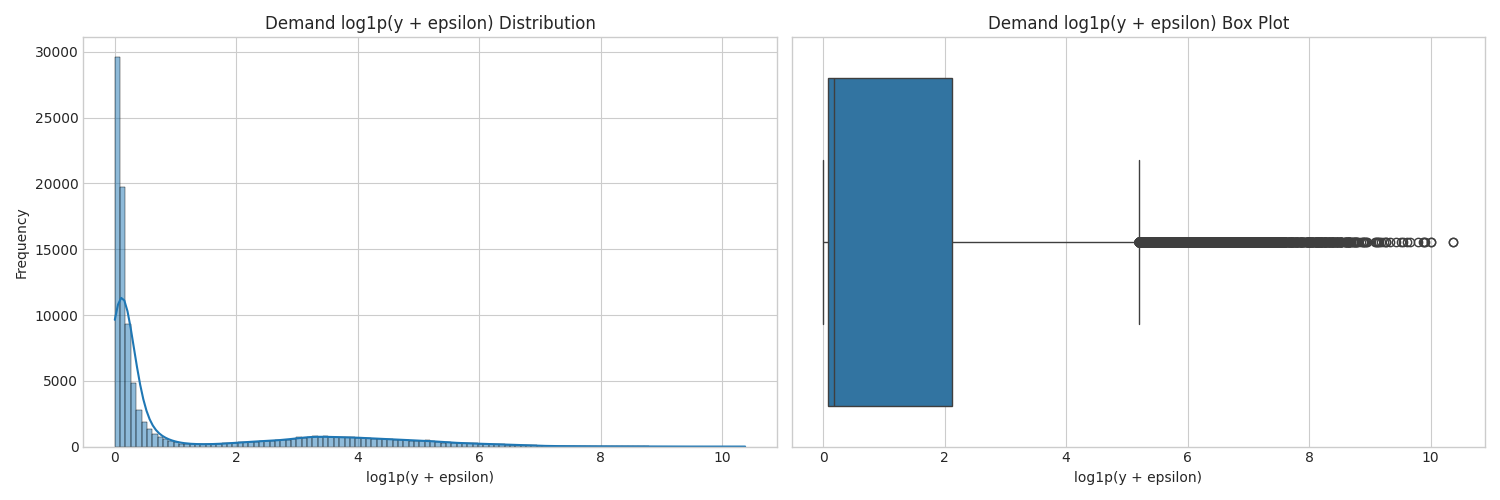
\includegraphics[width=\textwidth]{../plots/demand_y_distribution_log1p_scale.png}
        \caption{需求值 log1p 变换分布}
    \end{figure}
\end{frame}

\begin{frame}{需求时间序列特征}
    \frametitle{时间序列样本示例}
    \textbf{1. 小时周期性:}
    \begin{columns}
        \begin{column}{0.9\textwidth}
            \centering
            \begin{figure}
                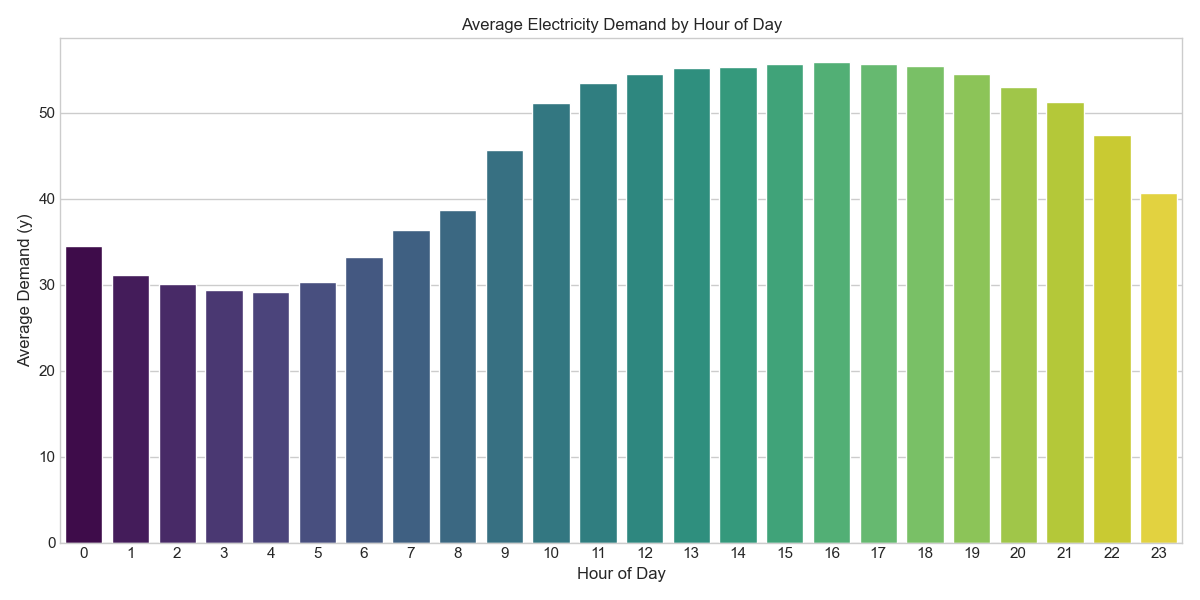
\includegraphics[width=\textwidth]{../plots/avg_demand_by_hour_spark.png}
            \end{figure}
        \end{column}
    \end{columns}
\end{frame}

\begin{frame}{需求时间序列特征}
    \textbf{2. 日周期性:}
    \begin{columns}
        \begin{column}{0.9\textwidth}
            \centering
            \begin{figure}
                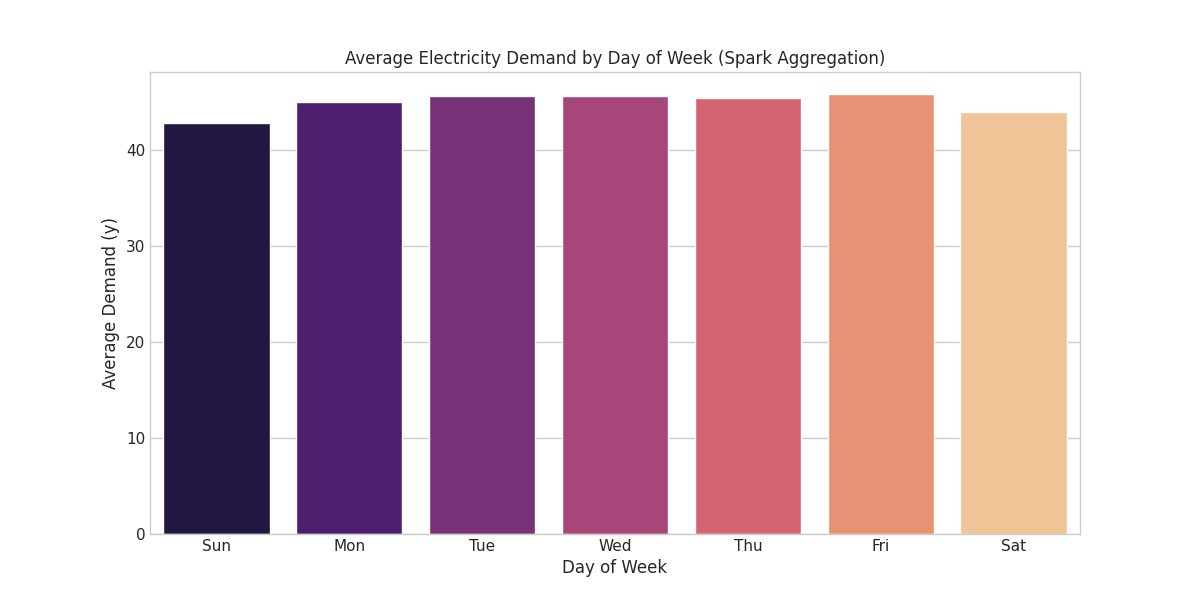
\includegraphics[width=\textwidth]{../plots/avg_demand_by_dayofweek_spark.png}
            \end{figure}
        \end{column}
    \end{columns}
\end{frame}

\begin{frame}{需求时间序列特征}
    \textbf{3. 月周期性:}
    \begin{columns}
        \begin{column}{0.9\textwidth}
            \centering
            \begin{figure}
                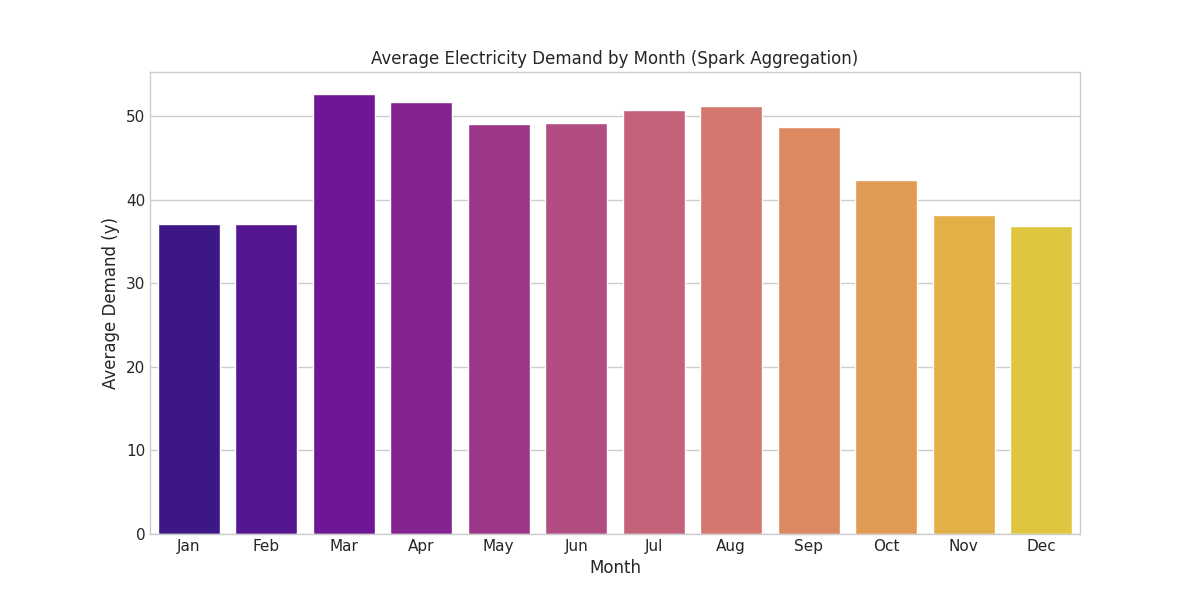
\includegraphics[width=\textwidth]{../plots/avg_demand_by_month_spark.png}
            \end{figure}
        \end{column}
    \end{columns}
\end{frame}


\begin{frame}{元数据分析}
    \frametitle{仪表与位置信息分布}
    \begin{itemize}
        \item \textbf{建筑类型 (Building Class):} 以 Residential (住宅) 为主 (~78\%),Commercial (商业) 占比较少 (~22\%)。
        \item \textbf{位置 (Location):} 大部分集中在 London, UK (~74\%),少量分布在葡萄牙 (PT) 和华盛顿特区 (Washington DC)。存在缺失位置信息 (~3.1\%)。
        \item \textbf{采样频率 (Freq):} 主要频率包括 30 分钟 (30T, ~73\%),1 小时 (1H, ~21\%) 和 15 分钟 (15T, ~5\%)。
    \end{itemize}
\end{frame}

\begin{frame}{天气数据分析}
    \frametitle{主要天气特征分布与时间特性}
    \textbf{主要分类特征分布:}
    \begin{columns}
        \begin{column}{0.7\textwidth}
            \centering
            \begin{figure}
                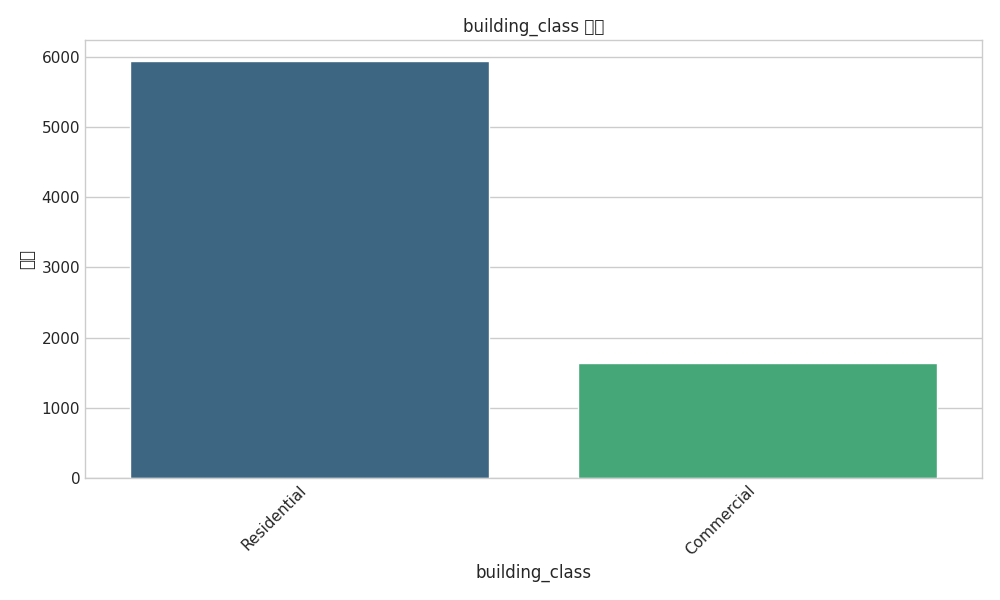
\includegraphics[width=\textwidth]{../plots/metadata_dist_building_class.png}
                \caption{建筑类型分布}
            \end{figure}
        \end{column}
        \begin{column}{0.3\textwidth}
            \centering
            \begin{figure}
                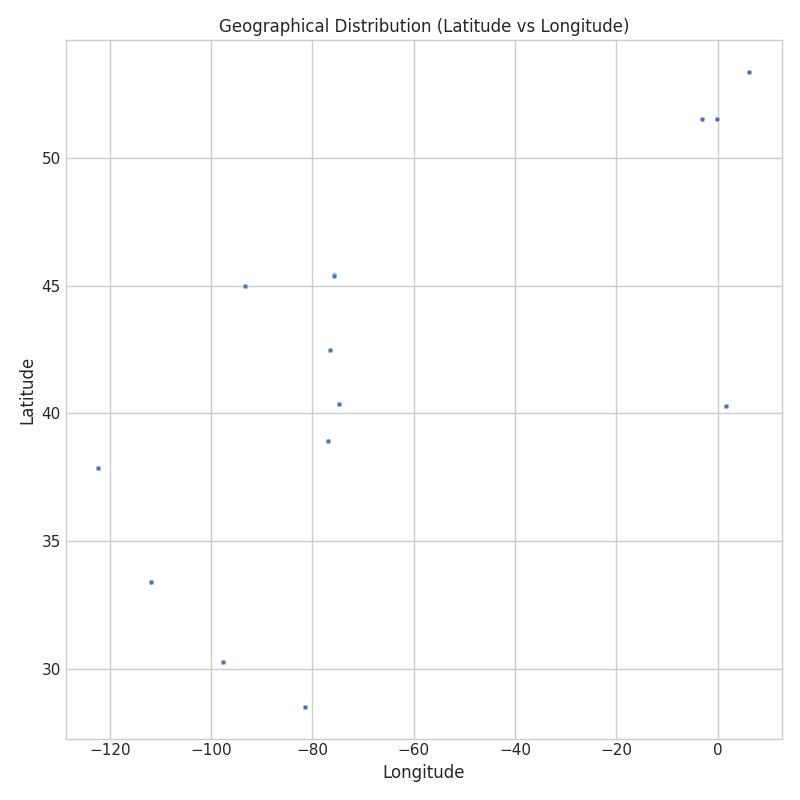
\includegraphics[width=\textwidth]{../plots/metadata_location_scatter.png}
                \caption{监测点地理位置}
            \end{figure}
        \end{column}
    \end{columns}
\end{frame}

\begin{frame}{天气数据分析}
    \begin{itemize}
        \item \textbf{数值特征分布:} 温度 (temperature\_2m) 近似正态分布,相对湿度 (relative\_humidity\_2m) 分布较广,降水 (precipitation) 存在大量零值 (零膨胀),风速 (wind\_speed\_10m) 呈右偏分布。
        \item \textbf{时间特性:} 天气数据主要以 1 小时为采样频率,记录规整。
    \end{itemize}
    \textbf{主要天气特征分布示例:}
    \begin{columns}
        \begin{column}{0.95\textwidth}
            \centering
            \begin{figure}
                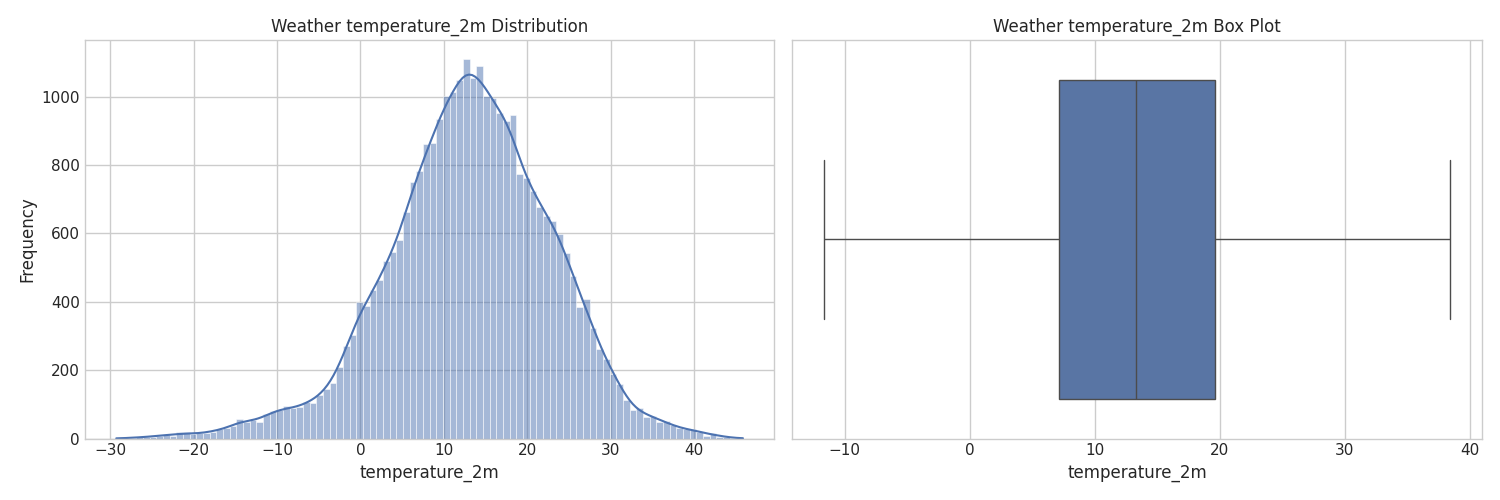
\includegraphics[width=\textwidth]{../plots/weather_distribution_temperature_2m.png}
                \caption{温度分布}
            \end{figure}
        \end{column}
    \end{columns}
\end{frame}

\begin{frame}{天气数据分析}
    \textbf{主要天气特征分布示例:}
    \begin{columns}
        \begin{column}{\textwidth}
            \centering
                \begin{figure}
                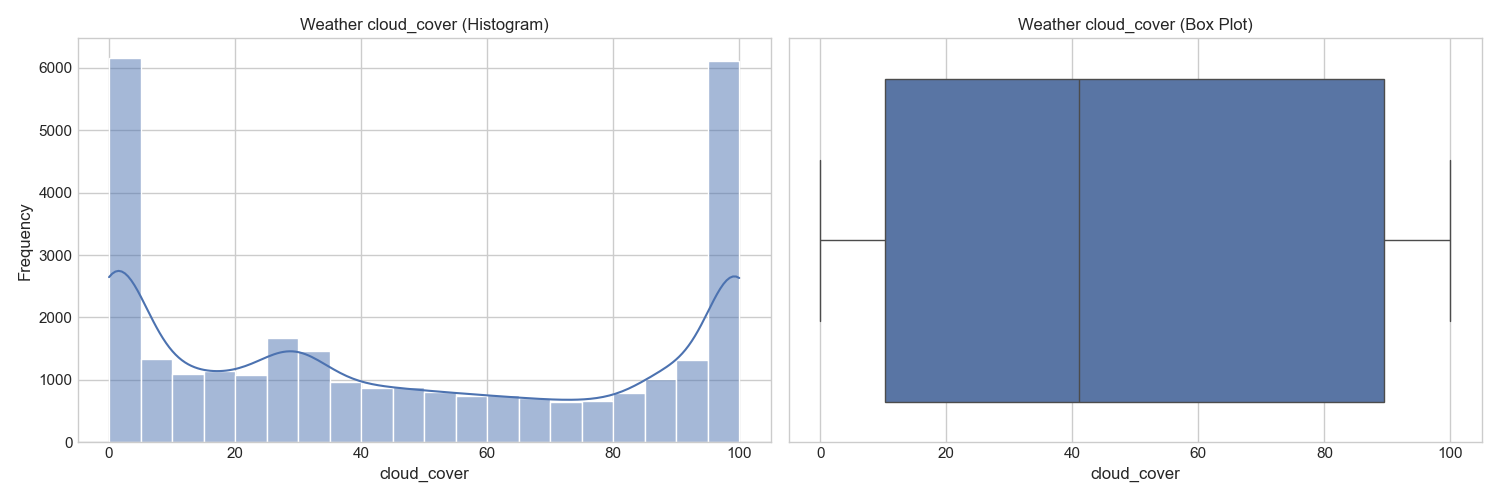
\includegraphics[width=\textwidth]{../plots/weather_distribution_cloud_cover.png}
                \caption{总云量分布}
            \end{figure}
        \end{column}
    \end{columns}
\end{frame}

\begin{frame}{需求与其他数据关系}
    \frametitle{建筑类型与天气的影响}
    \textbf{1. 需求与元数据关系 (建筑类型):}
    \begin{itemize}
        \item Commercial (商业) 建筑的电力需求量级通常显著高于 Residential (住宅),且波动更大。
    \end{itemize}
    \begin{figure}[H]
        \centering
        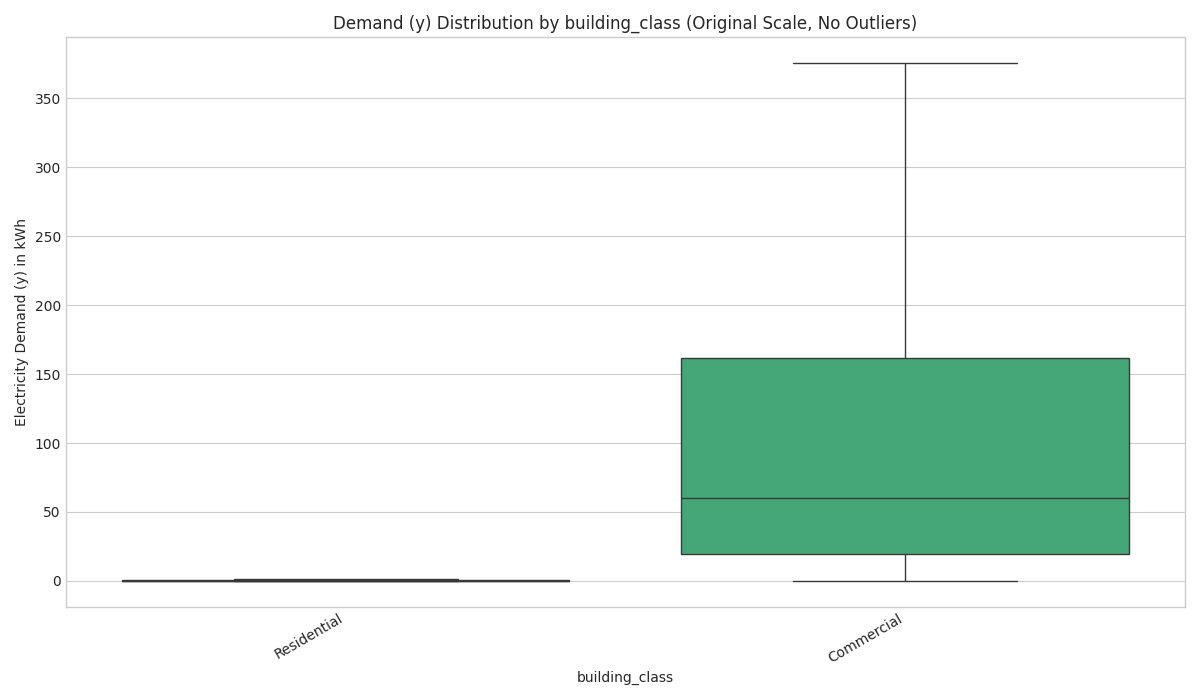
\includegraphics[width=0.6\textwidth]{../plots/demand_vs_building_class_boxplot_orig.png}
        \caption{需求 vs 建筑类型 (原始尺度)}
    \end{figure}
\end{frame}

\begin{frame}{需求与其他数据关系}
    \textbf{2. 需求与天气关系 (基于抽样合并):}
    \begin{itemize}
        \item 与 Temperature 呈弱正相关 (~0.03)。
        \item 与 Relative Humidity 呈中度负相关 (~-0.20)。
        \item 天气特征内部存在相关性,如温度与体感温度、云量特征之间。
    \end{itemize}
\end{frame}

% 5. 数据整合与频率匹配
\section{数据整合与频率匹配}

\begin{frame}{数据整合流程}
    \frametitle{多源数据合并步骤}
    \begin{enumerate}
        \item \textbf{加载与初步处理:} 加载 Demand, Metadata, Weather 数据。对 Demand 进行初步清洗(处理缺失和非正值)。
        \item \textbf{需求数据频率匹配:} 将不同频率的 Demand 数据重采样并聚合到统一的 \textbf{小时 (1H)} 频率,以匹配 Weather 数据。对于 freq < 1H 的数据,进行求和或平均聚合;对于 freq > 1H 的数据,考虑插值或保持原样(本项目聚合到小时)。
        \item \textbf{Weather 数据处理:} 清理 Weather 数据中的少量重复记录,确保每个 location\_id 在每个小时点只有一条记录。
        \item \textbf{数据合并:}
        \begin{itemize}
            \item 将重采样后的 Demand 数据与 Metadata 数据通过 unique\_id 进行左连接。
            \item 将上一步的结果与处理后的 Weather 数据通过 location\_id 和小时级 timestamp 进行左连接。
        \end{itemize}
    \end{enumerate}
\end{frame}

\begin{frame}{数据整合结果诊断}
    \frametitle{合并成功率与天气特征相关性}
    \begin{itemize}
        \item \textbf{合并成功率:} 约 1.73\% 的需求记录因元数据中缺少有效的 location\_id 或无法在天气数据中找到匹配的时间点,未能成功关联天气信息。其余数据 (~98.27\%) 成功合并。
        \item \textbf{天气特征内部相关性:} 合并后的数据集中,天气特征之间存在显著相关性,如下图所示。这在特征选择或模型选择时需要注意(如多重共线性)。
    \end{itemize}
\end{frame}

\begin{frame}{数据整合结果诊断}
    \begin{figure}[H]
        \centering
        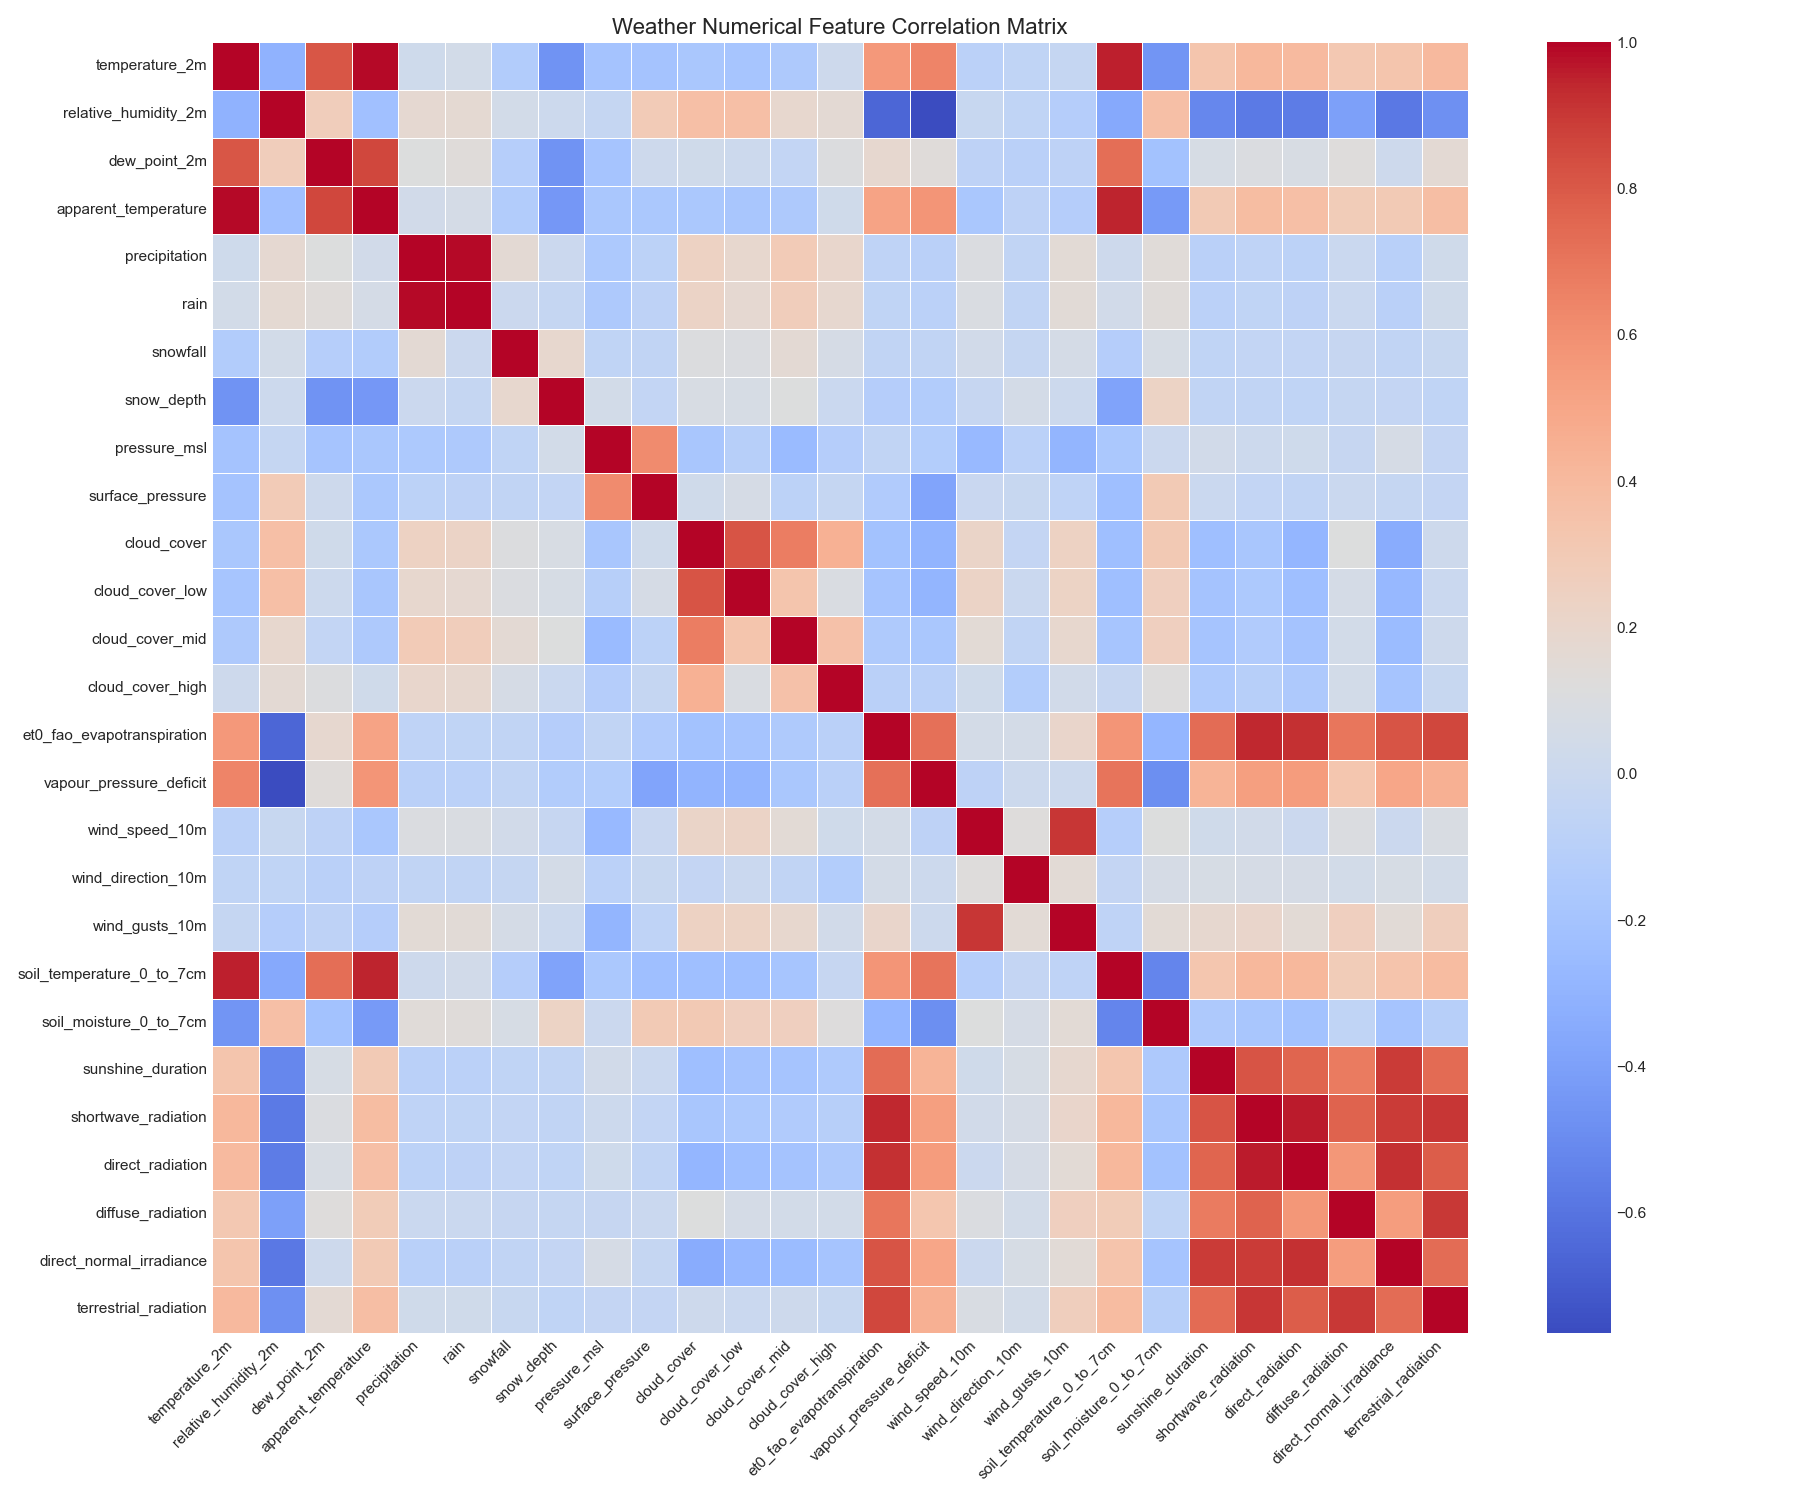
\includegraphics[width=0.7\textwidth]{../plots/weather_correlation_matrix.png}
        \caption{天气特征相关性矩阵}
    \end{figure}
\end{frame}


% 6. 特征工程
\section{特征工程}
\begin{frame}{特征工程}
    \frametitle{构建预测特征集}
    基于合并后的数据集,我们构建了以下类型的预测特征:

    \textbf{1. 时间特征:}
    \begin{itemize}
        \item 从 timestamp 中提取:年 (year),月 (month),日 (day),星期几 (dayofweek),年内天 (dayofyear),小时 (hour)。
        \item 考虑循环特征编码(如使用 sin/cos 转换小时和星期几)。
    \end{itemize}
    
    \textbf{2. 滚动窗口统计特征:}
    
    \begin{itemize}
        \item 基于历史电力需求 (y)。
        \item 在每个 unique\_id 的时间序列上计算。
        \item 考虑不同窗口大小 (例如,过去 3H, 12H, 24H, 168H)。
        \item 计算统计量如:均值 (mean\_lag\_Xh), 标准差 (std\_lag\_Xh), 最小值 (min\_lag\_Xh), 最大值 (max\_lag\_Xh)。
    \end{itemize}
\end{frame}
\begin{frame}{特征工程}
    \textbf{3. 原始/合并特征:}
    
    \begin{itemize}
        \item 来自 Metadata:building\_class, location\_id, freq 等 (需进行编码)。
        \item 来自 Weather:temperature\_2m, relative\_humidity\_2m, apparent\_temperature 等。
    \end{itemize}
    \textbf{缺失值处理:} 移除了目标变量 y 缺失的行;滚动特征计算初期产生的缺失值也需处理(例如,移除或使用插补)。
    
    \textbf{输出:} 最终特征集按年/月分区存储为 Parquet 文件 (data/features.parquet)。
\end{frame}


% 7. 总结与下一步
\section{总结与下一步}

\begin{frame}{总结}
    \frametitle{主要发现回顾}
    \begin{itemize}
        \item \textbf{数据特性:} 规模大,包含需求、元数据、天气多源信息;需求分布高度右偏,存在非正值和异常值。
        \item \textbf{数据质量:} 存在少量 y 缺失和元数据位置信息缺失,天气数据有少量重复(已处理)。
        \item \textbf{关系:} 建筑类型(商业需求显著高于住宅)和天气(温湿度)与电力需求存在关联。天气特征内部有相关性。
        \item \textbf{时间模式:} 需求表现出清晰的日、周、年度周期性。不同数据源的时间频率不匹配已通过重采样到小时频率解决。
        \item \textbf{处理过程:} 利用 Spark 有效处理了大规模数据;通过抽样和可视化进行了深入的 EDA;成功整合了异构数据源并构建了初步的时间、滚动、原始特征集。
    \end{itemize}
\end{frame}

\begin{frame}{模型训练结果与初步解读}
    \frametitle{初步模型评估与结论}
    使用了基于小时频率聚合并进行特征工程的数据集 (data/features.parquet) 训练了两个 Spark MLlib 回归模型,并在测试集上进行了评估 (基于时间分割)。

    \textbf{1. MLlib 线性回归 (Linear Regression)}
    \begin{itemize}
        \item 测试集 RMSE: 73.81
        \item 测试集 MAE: 5.86
    \end{itemize}

    \textbf{2. MLlib GBT 回归 (Gradient Boosted Trees Regression)}
    \begin{itemize}
        \item 测试集 RMSE: 175.40
        \item 测试集 MAE: 54.04
    \end{itemize}
\end{frame}

\begin{frame}{模型训练结果与初步解读}
    \frametitle{GBT 模型特征重要性 (Top 10):}
    \begin{itemize}
        \item y\_rolling\_max\_3h (近期最大需求): 0.1882
        \item y\_rolling\_stddev\_48h (过去 2 天需求波动): 0.1161
        \item y\_rolling\_stddev\_6h (近期需求波动): 0.0969
        \item hour (小时): 0.0946
        \item y\_rolling\_min\_48h (过去 2 天最小需求): 0.0908
        \item y\_rolling\_min\_168h (过去 1 周最小需求): 0.0888
        \item y\_rolling\_stddev\_3h (极近期需求波动): 0.0519
        \item soil\_temperature\_0\_to\_7cm (土壤温度): 0.0470
        \item y\_rolling\_stddev\_24h (过去 1 天需求波动): 0.0394
        \item year (年份): 0.0338
    \end{itemize}
\end{frame}

\begin{frame}{模型训练结果与初步解读}
    \textbf{初步结论与解读:}
    \begin{itemize}
        \item \textbf{模型性能对比:} 出乎意料地,简单的线性回归模型在测试集上的表现 (RMSE=73.81, MAE=5.86) 显著优于梯度提升树回归模型 (RMSE=175.40, MAE=54.04)。这表明当前的 GBT 模型可能存在调优不足、过拟合或特征处理等问题,需要进一步检查。
        \item \textbf{特征重要性:} GBT 模型的结果显示,近期历史用电量相关的滚动统计特征 (特别是过去 3 小时的最大值、不同时间窗口的标准差和最小值) 是最重要的预测因子。时间特征 (小时、年份) 也具有较高的重要性。土壤温度作为一个天气相关特征也进入了 Top 10。
        \item \textbf{下一步:} 需要深入分析 GBT 模型性能不佳的原因,并考虑优化模型参数或尝试其他模型。线性回归的较好表现可能得益于其简单性或对当前特征集的适应性,但也需警惕其可能无法捕捉复杂的非线性关系。
    \end{itemize}
\end{frame}

\begin{frame}{后续步骤 (续)}
    \frametitle{下一步:模型结果分析与改进}
    \begin{enumerate}
        \item \textbf{模型结果分析:}
        \begin{itemize}
            \item 分析已训练模型的性能(RMSE, MAE)。
            \item 检查特征重要性,理解哪些特征对预测贡献最大。
            \item 进行误差分析,了解模型在哪些情况下表现不佳。
        \end{itemize}
        \item \textbf{模型改进或探索其他模型:}
        \begin{itemize}
            \item 尝试更复杂的模型架构或算法。
            \item 探索特征工程的其他方法,如交互特征或更高阶统计量。
            \item 考虑使用时间序列模型,如 ARIMA, Prophet, LSTM 等。
        \end{itemize}
        \item \textbf{模型评估与选择:}
        \begin{itemize}
            \item 在验证集上评估不同模型的性能。
            \item 选择最优模型并在测试集上进行最终评估。
        \end{itemize}
        \item \textbf{预测与应用:} 使用最优模型对未来的电力需求进行预测。
    \end{enumerate}
\end{frame}

\end{document}
